\section{Evaluation}
\label{sec:eval}

\subsection{Study of the effect of garbage collection on Spark runtime}
\paragraph{}
Our first set of experiments were conducted to understand the effect of
memory pressure on applications by quantifying the impact of garbage
collection when running a PageRank application on Spark. The high level
questions that we wanted to answer are as follows:

\begin{enumerate}
\item What is a good strategy of scaling big-data applications? (more
    cores, less memory per core versus less cores, more memory per core) 
\item What is the impact of managed runtimes on application throughput?
\item What is the more fundamental problem with the way memory is managed
    by runtime engines when running big-data applications on Spark?
\end{enumerate}

\paragraph{Experimental Setup:}
The experiments were conducted on machines with Intel Xeon processors
running at clock frequency of 2.66GHz, with 4 cores per processor, and
16 GB of DRAM. Each machine runs Linux version 2.6.18 with L1 cache
size of 32K.

\paragraph{Experimental 1:}
The experiments are conducted on the following five different configurations:
\begin{itemize}
\item Configuration 1 (15W, 1G): The configuration consists of 15 worker nodes, each with 1 GB of memory.
\item Configuration 2 (10W, 1G): The configuration consists of 10 worker nodes, each with 1 GB of memory.
\item Configuration 3 (5W, 2G):  The configuration consists of 5 worker nodes, each with 2 GB of memory.
\item Configuration 4 (2W, 5G):  The configuration consists of 2 worker nodes, each with 5 GB of memory.
\item Configuration 5 (1W, 7.5G):The configuration consists of 1 worker node, each with 7.5 GB of memory.
\end{itemize}

\paragraph{}
The application we run is the vanilla PageRanking algorithm provided
with the Spark library. The dataset that we take describes a network
which was collected by crawling Amazon website. It is based on the
\textit{Customers Who Bought This Item Also Bought} feature of the
Amazon website. If a product $i$ is frequently co-purchased with product
$j$, the graph contains a directed edge $i \rightarrow j$
\cite{leskovec}. It includes a graph of \textit{403394 nodes} with
\textit{3387388 nodes}. The data is around \textit{50MB} in size. The
page ranking algorithm was run for \textit{10 iterations}.

Table \ref{tab:table1} lists out the running times, along with the
overheads due to the garbage collector for different configurations.

\begin{table}[h!]
\begin{tabular}{| c | c | c | c |}
\hline
Configuration  & Application Run  &  \% Overhead  \\ 
& Time (in ms) & due to GC \\ \hline
15W, 1G & 428,245  & 33\% \\ \hline
10W, 1G & 414,742 &  30.5\% \\ \hline
5W, 2G & 216,320 & 23\%  \\ \hline
2W, 5G & 152159 & 15.29\% \\ \hline
1W, 7.5G & 164893 & 8.45\% \\ \hline
\end{tabular}
\caption{Comparison of the overhead in throughput due to garbage collection for different configurations}
\label{tab:table1}
\end{table}

\paragraph{Analysis of results:}
Fig. \ref{fig:exp4} shows a relative comparison of the overall
throughput from the cluster under different configuration settings. Fig.
\ref{fig:exp4_2} shows a relative comparison of the impact of garbage
collection on the cluster under these configuration settings. We can
observe that garbage collection has a detrimental effect on the overall
running time of the application. For a configuration of 2 nodes with 5
GB of memory per server, the overall running time of the application
increased by 16\%, whereas for a setup of 15 workers with 1 GB of memory
on each server the overall running time of the application was reduced
by 33\%. 

\begin{figure}[!ht]
\caption{Comparison of application runtime for different configurations}
\label{fig:exp4}
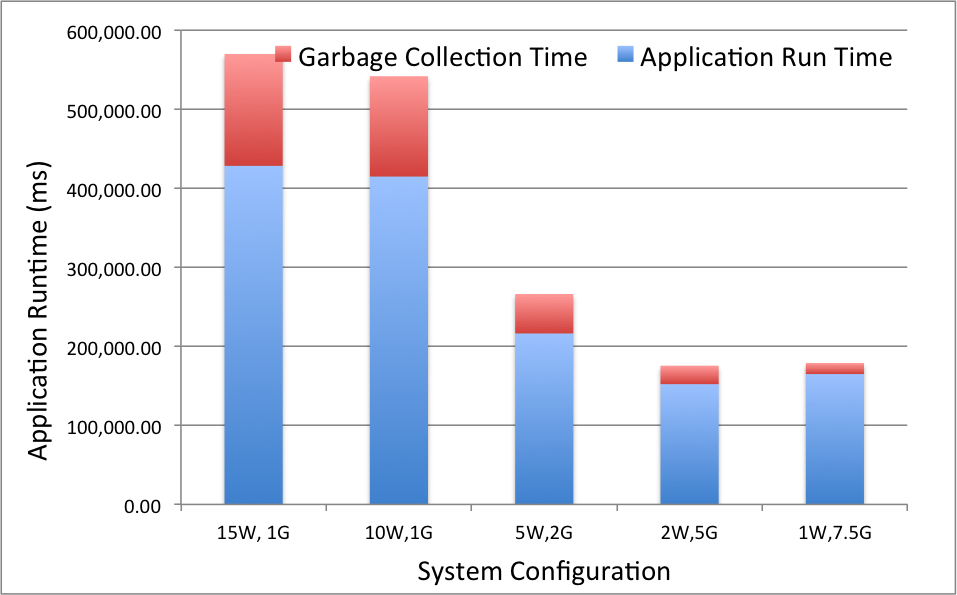
\includegraphics[scale=0.50]{./images/exp4.png}
\end{figure}

\begin{figure}[!ht]
\caption{Comparison of relative affect of garbage collection on application runtime for different configurations}
\label{fig:exp4_2}
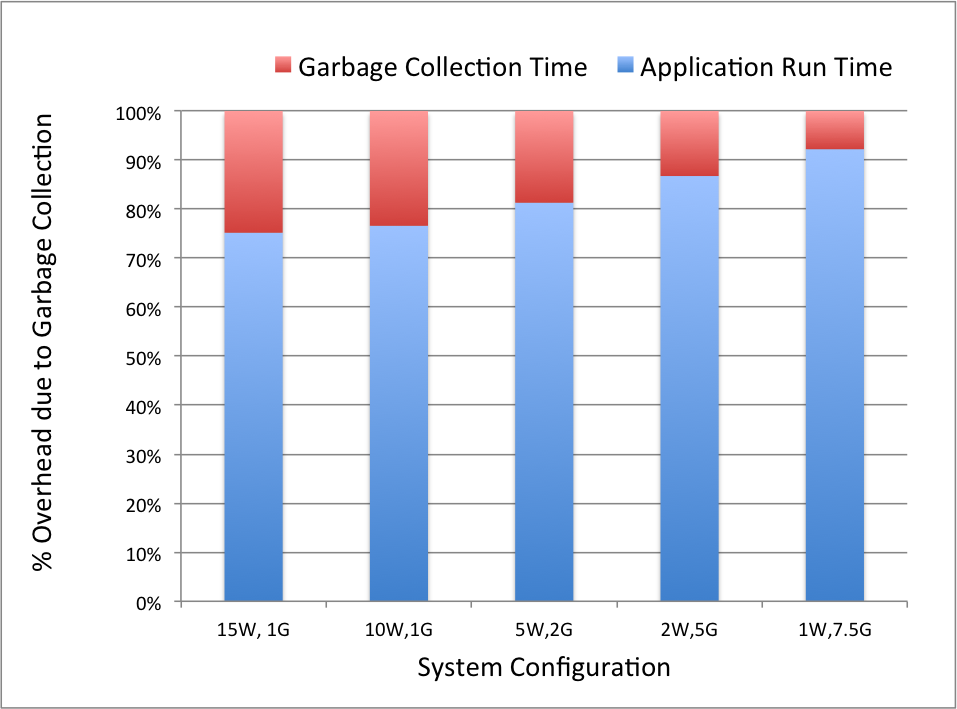
\includegraphics[scale=0.50]{./images/exp4_2.png}
\end{figure}

\begin{figure}[!ht]
\caption{Comparison of application runtime for successive tasks for two different configurations}
\label{fig:exp5}
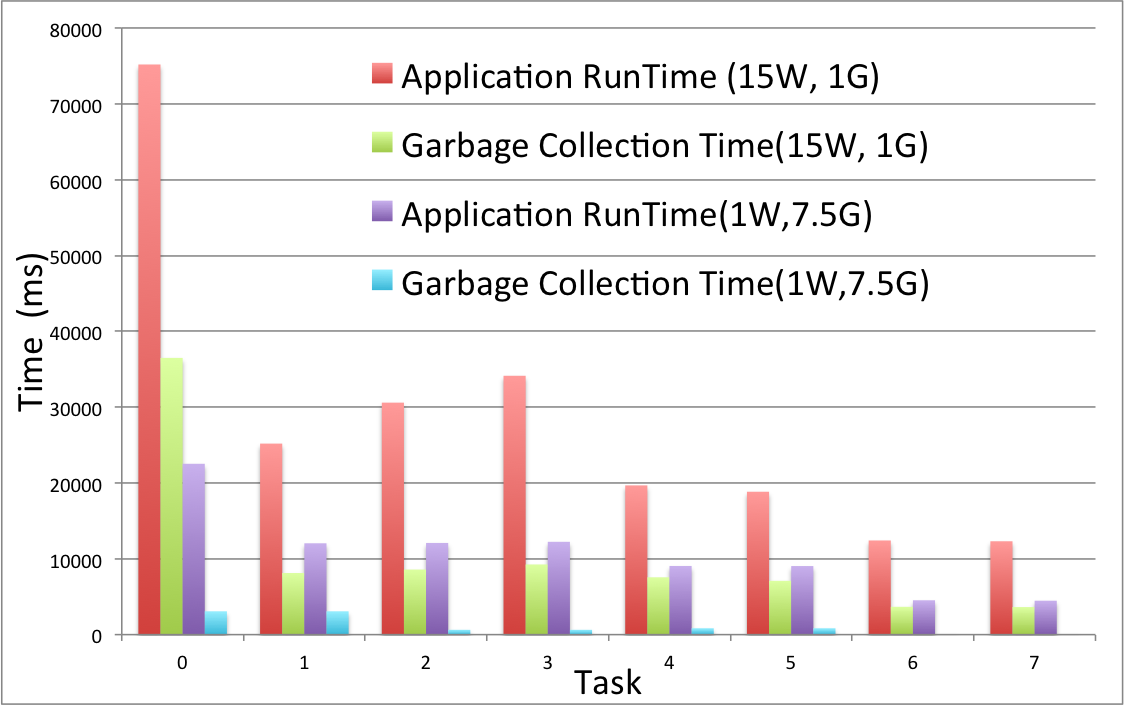
\includegraphics[scale=0.40]{./images/exp5.png}
\end{figure}

\paragraph{}
There are several reasons that explain the above behaviors.  Firstly,
Spark is an in-memory runtime application. It requires extensive amounts
of memory for storing intermediate data such as when deserializing data
read from the storage layer, maintaining cache of RDDs, lineages of RDDs
etc. Larger memory requirements creates extra memory pressure triggering
frequent garbage collection. Therefore the overall throughput of the
application decreases. Secondly, in order to scale the application, when
the number of nodes in the cluster is increased, the synchronization
costs due to communication over the network and secondary storage causes
additional overhead.  An intuitive conclusion one can derive from the
above set of experiments is that in order to scale memory-intensive
applications, horizontal scaling may not be as effective as scaling
resources on individual nodes. 

%%%%%%%%%%%%%%%%%%%%%%%%%%%%%%%%%%%%%%%%%%%%%%%%%%%%%%%%%%%

\subsection{Study of object-level access patterns within Spark} 
\paragraph{} In order to answer the second question, we took a dummy
application in Spark that calculates the value of Pi on a local machine. 

\paragraph{Objective:}
The objective of the experiment is to measure the spectrum of object
level accesses when running a baseline Spark application that does
minimal work. 

\paragraph{Experimental Setup:} 
The experiments were conducted on Intel(R) Xeon(R) CPU E3-1230 V2
machines running at a clock frequency of 3.30GHz with 8 cores with L1
cache size of 32K. For the experiment we used 512MB of memory.

\paragraph{Analysis of results:} 
The results we report are for a specific period of time for which the
application runs, since our interception mechanism (as explained in
Section \ref{sec:design}) can approximate object accesses within a
single evacuation cycle of G1 garbage collection.

Fig. \ref{fig:exp6} shows a histogram of the object-level accesses
of different component objects within the Spark application. The results
indicate a remarkable heavy-tailed object-level access pattern: within
the specified period of time, around 45,000 objects were live in the young
generation of the application; out of these, around 1,000 objects
(nearly 2\%) had an access count of over 1,000, which we labeled as
\emph{hot objects}, and contribute for nearly 58\% of the total accesses
within the survivor and eden regions.
%Nearly 17\% of the overall accesses derived from 0.02\% of the total objects.
On the other hand, nearly 3\% of the overall accesses are coming for
50\% of the objects in the specified regions of the memory.
These numbers clearly indicate that the object-level access patterns
within applications are extremely heavy-tailed. 

\begin{figure}[!ht]
\caption{Histogram of object accesses for different objects for a Spark Application}
\label{fig:exp6}
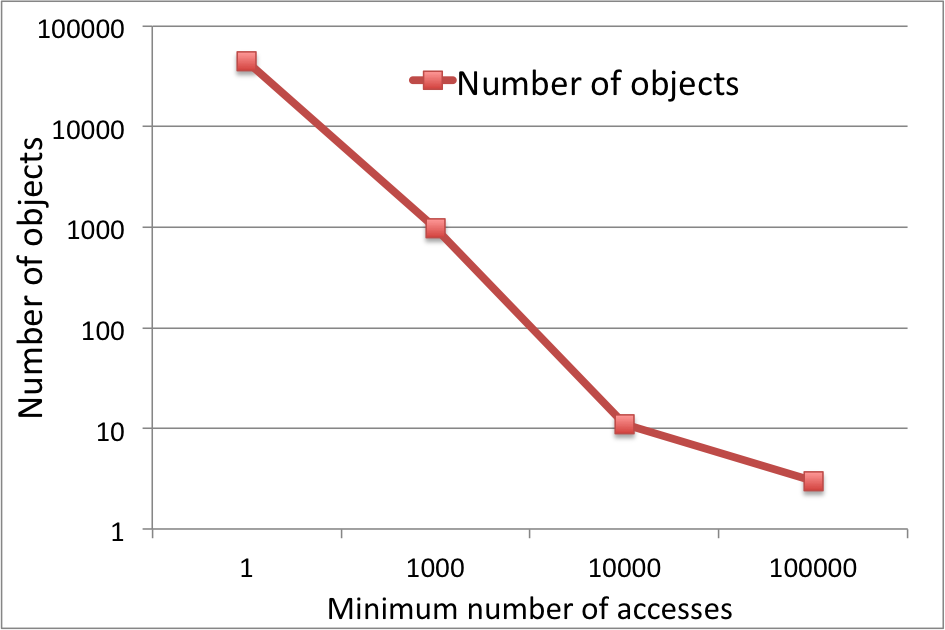
\includegraphics[scale=0.50]{./images/exp6.png}
\end{figure}

\paragraph{}
Here we give three reasons to explain the heavy tail in the distribution
of object level accesses pattern.
Firstly, accesses to large arrays of objects (such as RDDs) will have
especially high numbers since each access of an object in an array is
also an access to that array (much like a container of objects).  Such
arrays can be classified as hot objects in the object space.
Secondly, instances of objects that contain utility functions such as
methods for compressing, polling the network interfaces, DOM parsing
have large access counters. Due to their generic functionality, these
objects could become the frequent access spots.
Thirdly, a very large collection of objects (nearly half of all the
objects) such as classes for caching root names might get accessed once
and be used only at certain specific intervals, such as that at a task
start up for looking up the addresses of the different workers.  These
\emph{cold objects} show the low-usage access pattern. 
To conclude, most of the data objects likely to be frequently accessed
are arrays or utility functions (such as worker queue, XML document
handlers, symbol table entry handlers, loggers, etc.)
The objects that are less frequently
accessed are temporary objects, such as method objects, strings, classes
for caching root names, object for looking up the MIME types (used for
inspecting object headers), objects created for storing symbol tables
for compilers, parsers, etc.

\paragraph{}	
The long-tail distribution of access patterns unearths a potential
problem in contemporary memory management system design. Current virtual
memory systems have a page based abstraction for managing in-memory application
data, while data residing on the same pages might not
always have very good ``access similarity''. Paging, therefore, by virtue
of its underlying design, cannot capture the access level semantics of
applications at an appropriate granularity. This experiment provides us with
useful insights and helps further our understanding of the underlying
fundamental problems within current memory management system designs.

%%%%%%%%%%%%%%%%%%%%%%%%%%%%%%%%%%%%%%%%%%%%%%%%%%%%%%%%%%%

\subsection{Study of Indexed RDDs effectiveness}
\paragraph{Objective:} We observe that while the design of RDDs supports
caching and faster recovery through lineages, it lacks certain
capabilities. Besides, RDDs inherently support operations on datasets
which consist of pairs of key and values. We posit a natural extension
to the design of RDDs using range partitioned indexes on keys. This
experiment answers the following three questions:

\begin{enumerate}
\item How to improve the efficiency of running queries on
    semi-structured data (such as database logs, page-visit history)? 
\item What are better schemes of indexing larger datasets using RDDs?
\item How well can a generic indexing scheme based on range partitioning
    scale? 
\end{enumerate}

\paragraph{Experimental Setup:} The experiments were conducted on
machines with Intel(R) Xeon(R) CPU E3-1230 V2 running at a clock
frequency of 3.30GHz, with 8 processor cores, with 32GB of DRAM size.
Each machine runs Linux version 3.11.10 with L1 cache size of 32K.  The
experiments were run on a cluster of 3 nodes connected with 1 Gbps NICs
arranged on a single rack. The Spark setup consisted of 6 workers (2 on
each machine) and 1 master. Each of the workers was configured with 8GB
of memory and the master had 2 GB of memory.  The master physically
locates on the same machine as one of the workers. The tests were run
using using the Spark shell interface.  The experiments were conducted
on Hadoop file system (version 2.2.0).  The block size was set to
default 256MB. The Hadoop master and data nodes were set up on the same
machine.

\paragraph{Datasets:} For the experiments we used page view logs from
Wikimedia dumps \cite{wikimedia}. Wikipedia publishes page view
statistics every month.  The following is an example of the data:\\
\texttt{fr.b Special:Recherche/Achille\_Baraguey\_d\%5C\%27- Hilliers 1
624} \\
All data items are in this 4-column format. The first column
\texttt{fr.b} denotes the project name; the second column is the title
of the page retrieved; the third column is the number of requests, and
the fourth column is the size of the content returned.
In our experiments, we use the project names as the keys and the rest
parts of the lines as the values that need to be retrieved from the
underlying distributed file system.  We use two different collection of
data (10GB and 25GB), approximating 5 months and 1 years of data
respectively, with nearly 300 million and 730 million records. 

\paragraph{Experiment 3:}
For the experiments we run five different queries and measure the
overall time it takes for the queries to complete. 

Fig. \ref{fig:exp7} shows a comparison of three different configurations
when running the queries on 10GB file. VSpark denotes queries on vanilla
Spark using unindexed RDDs; ISpark\_C (Indexed Spark Coarse-Grained
Partitioned) denotes RDDs with 320 partitions; and ISpark\_F (Indexed
Spark Fine-Grained Partitioned) denotes RDDs with 1280 partitions. While VSpark
takes 87 seconds to complete, the average time for a positive query (a
query that matched keys in the file) on ISpark\_C was around 37 seconds.
Using more fine grained partitioning ISpark\_F, the average time lowers
down to 11 seconds. It is also worth noting that for queries that miss
match, the result is returned in less than one second. The reason is
that the range partitioning mechanism can pre-determine the set of RDDs
on which the query needs to be run on, which helps reduce the overall
computation that needs to done for filtering records. Besides, the
communication cost over the network also gets reduced.  For queries
result in a miss, the master can instantaneously return an empty result
by just looking up the key ranges mapping and determining that certain
key is outside the range of all the partitions.

\begin{figure}[!ht]
\caption{Comparison of query completion times between Spark, Spark Coarse-grained and Spark Fine-grained partitioned for a 10GB file}
\label{fig:exp7}
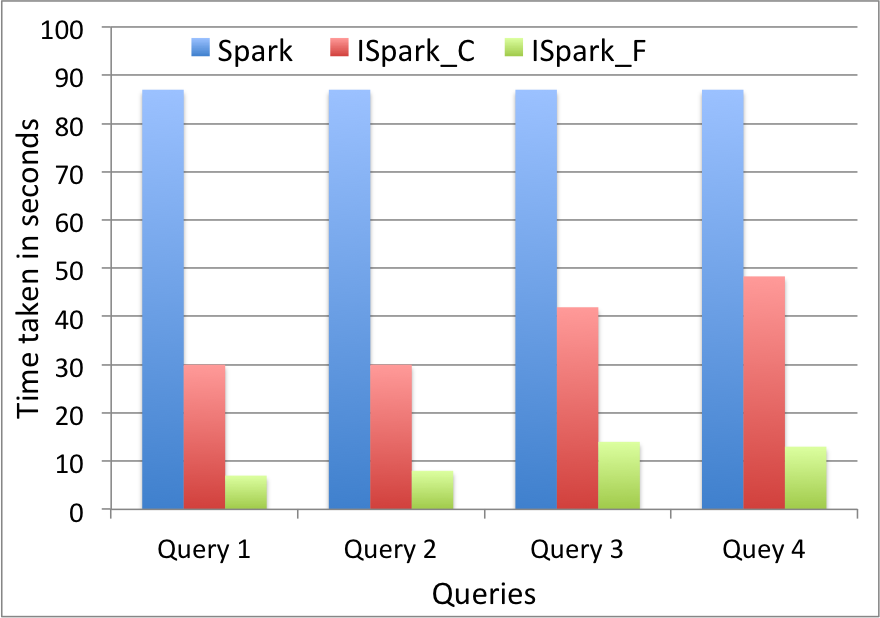
\includegraphics[scale=0.50]{./images/exp7.png}
\end{figure}

\paragraph{}
Fig. \ref{fig:exp8} shows a comparison of the three aforementioned
configurations when running the queries on 25GB file. The number of
partitions for ISpark\_C is 1,572, and that for ISpark\_F is 10,000.
While VSpark takes 220 seconds to complete, the average time for a
positive query using ISpark\_C is around 49 seconds. Using, more fine
grained partitioning ISpark\_F, the average time lowers down to 9
seconds. We can observe that while VSpark scales poorly as the size of % To be changed: Spark scales poorly
data increases, indexes helps the filtering query to scale in a more
scalable manner. With more fine grained partitioning, we were able to
reduce the overall query time for a 25GB over 10GB. However, limited by
the master node memory, we cannot further increase the number of
partitions. For future experiments, in order to scale up, we can
maintain a separate indexing server that can cache indexes and return
the set of RDDs on which a query has to be run. 

\begin{figure}[!ht]
\caption{Comparison of query completion times between Spark, Spark Coarse-grained and Spark Fine-grained partitioned for a 25GB file}
\label{fig:exp8}
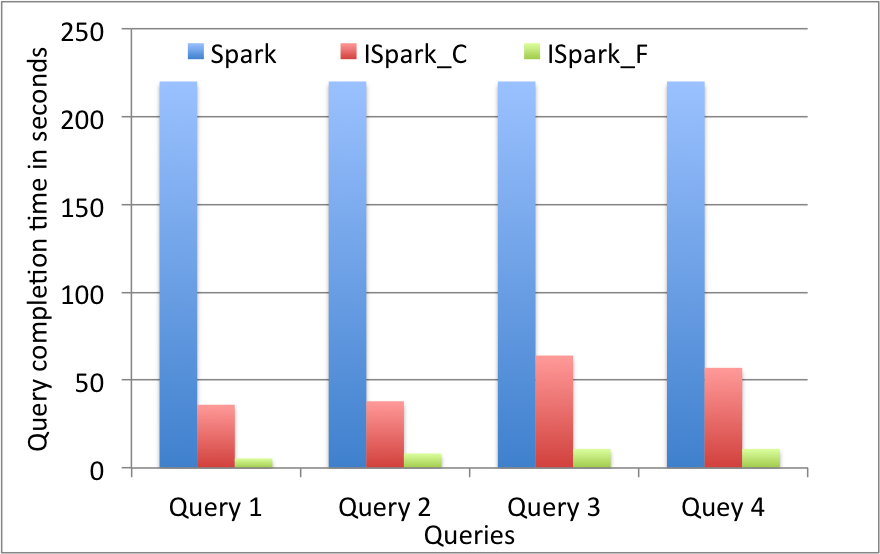
\includegraphics[scale=0.50]{./images/exp8.png}
\end{figure}

\paragraph{}
Fig. \ref{fig:exp9} shows the overall time it takes for the indexing
mechanism to initialize the partition metadata on the RDDs. The
partitioning schema scales in accordance with the filtering mechanisms
since the all the set of records have to be filtered. However, since
this is a one-time cost, the cost will be amortized with a batch of
queries. Besides, the time it takes to build indexes does not increase
by a large amount as the number of partitions increases. Therefore, fine
grained indexing can be very useful, as long the master has sufficient
memory to hold the index.

\begin{figure}[!ht]
\caption{Comparison of index creation time}
\label{fig:exp9}
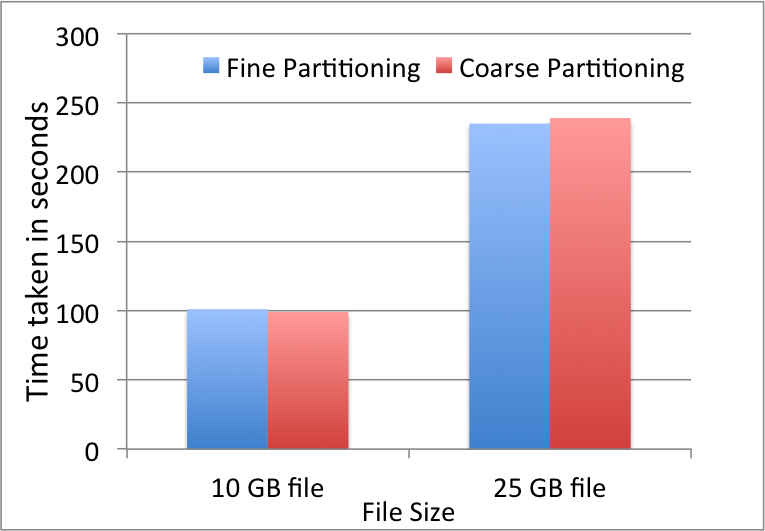
\includegraphics[scale=0.50]{./images/exp9.png}
\end{figure}
